%!TEX root = ../deco_star.tex
\section{Introduction}
Pattern generation in computer graphics provides vast amounts of precise and quickly generated digital content. However, despite over three decades of research, supporting artists with meaningful digital tools for creative content generation, \rev{Referencing a visual example:}{as for example needed for ornamental pattern designs (\Cref{fig:historic_examples})}, is an ongoing research challenge. Most solutions focus on adding singular features and control mechanisms, such as an example-based control or a brush, on an algorithmic level. Little attention, however, is paid to an overall creative workflow, which needs to strike a balance, giving users as much power as needed without burdening them with unwanted details. Often, techniques are claimed to be artist-controllable but are less often proven to be so.

This may be a consequence of research often being executed without direct and continuous collaboration with artists and without the support of large-scale user studies. Algorithms and methods are being developed mostly to add to state of the art, such as building on recent progress in deep learning research, and there is little common understanding in the research community regarding what artist needs are and how mechanisms are validated.

Recent surveys have covered 3D generation in much detail, focusing on  world building~\cite{smelik_2014_aso, aliaga_2016_ipm}, terrain modeling~\cite{galin_2019_aro} and game-specific approaches~\cite{hendrikx_2013_pcg, togelius_2011_sbp}. In this report, we review recent advances in 2D pattern generation. 

The underlying regularity of 2D pattern designs is based on a repetitive and balanced distribution of elements, usually following hierarchical structures. These characteristics can be efficiently implemented by procedural approaches that arrange elements in space according to generative rules~\cite{stava_2010_ipm}. The primary motivation of, for example, inverse procedural models is to free the artist from tedious, non-inspiring, and repetitive tasks. Computational generation techniques are not only an easement, but they also perform in a potentially more precise and less error-prone way than a human artist. Hence, procedural representations are an ideal basis for creative pattern generation. However, the creative demands of, for example, laying out space-specific designs and placing visual accents must also be considered. Procedural models must be augmented, and different approaches must be unified to enable the control and quality of manual creation and the efficiency and accuracy of computation~\cite{gieseke_2017_ooo}. 

We review recent advances in 2D pattern generation and discuss procedural models, data-driven generation, and design-specific pattern generation. As theoretical grounding, we classify control mechanisms and their characteristics from the perspective of an artist from global to local and from automatic to manual, with varying levels of abstraction for their handling. As a basis for a discussion of the capabilities of control mechanisms in a creative process and their potential for innovative creation, we review the literature on creativity and summarize aspects that can help to understand such capabilities in the context of computer graphic publications.

We organize contemporary techniques by design areas and the visual features they enable. We further group related work by commonly used control types. Then, we specifically analyze for each reference the offered control for an artist. 
We conclude the review with a discussion of the creative means for the different control mechanism types. With this survey, we hope not only to categorize and summarize state of the art meaningfully but also to contribute to a shared vocabulary and a foundation for making it more accessible in the future to incorporate artists and creative tasks into algorithmic content creation pipelines.

\begin{figure}
    % \centering
        %TODO: Replace with png for submission
        \revimage{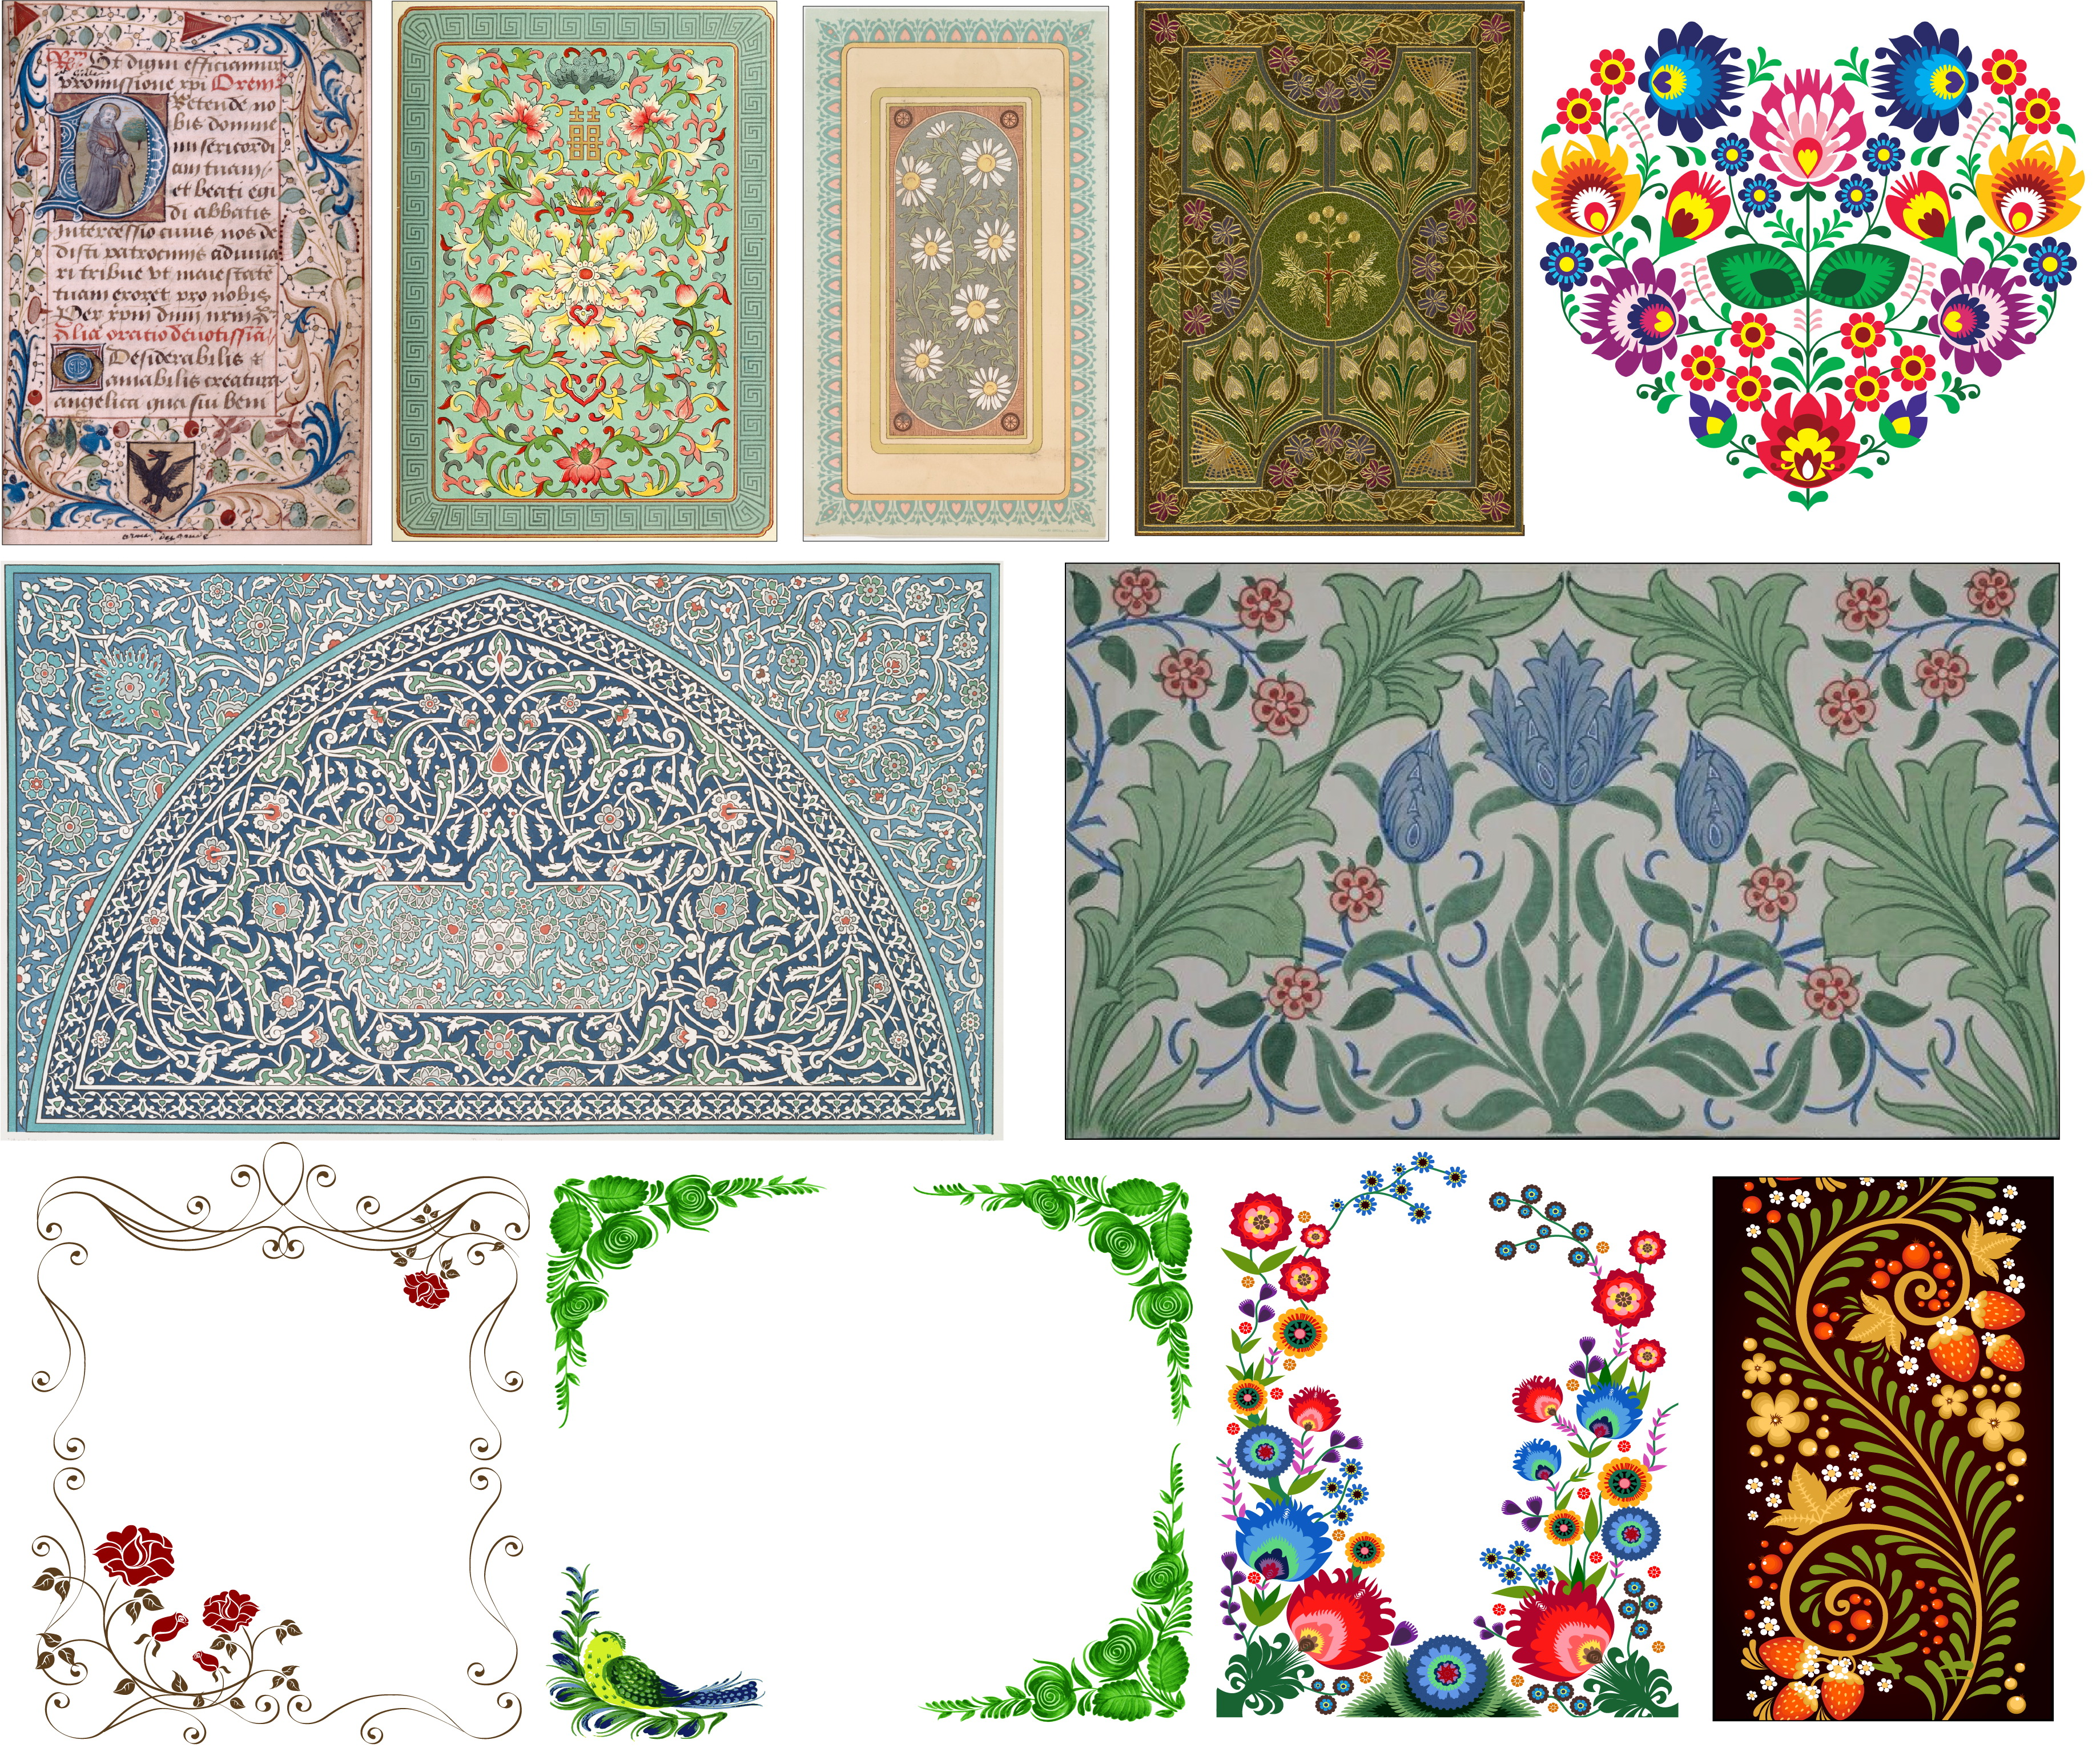
\includegraphics[width=1.0\columnwidth]{figures/historic_examples/examples.jpg}}
        \caption[Historic pattern examples]{\label{fig:historic_examples} Historic examples for creative pattern designs and ornamentation. Places of origin from left to right, top to middle row:  France, China, USA, UK, Poland, Egypt, UK (cutout of a tiled pattern). Bottom row: recent commercial examples. This figure is adapted from~\cite{gieseke_2017_ooo}, image sources: [1-10].}
\end{figure}
